\documentclass{beamer}
\usepackage{graphicx}
\usepackage{amsmath}
\usepackage{bm}
\graphicspath{{Images/}}
\mode<presentation>
\title{Introduction to the Finite Element Method}
\institute{NONE}
\date{2017-05-16}

\begin{document}
\frame{\titlepage}
\begin{frame}
	\frametitle{Overview} 
	\tableofcontents
\end{frame}
\section{Introduction}
\begin{frame}{Introduction}
\begin{block}{Disclaimer}
	This is meant to be a brief overview of Computational Structural and Fluid Dynamics.
	All of this Material is taken from:
	\begin{enumerate}
		\item \underline{Nonlinear Finite Elements for Continua and Structures} by Ted Belytschko 
		\item \underline{Computational Gas Dynamics} by Culbert Laney
	\end{enumerate}
\end{block}
\begin{block}{Topics To Be Covered}
\begin{itemize}
	\item Lagrangian and Eularian Frames
	\item Continuum Mechanics Overview
	\item Conservation Equations
	\item Weak Forms and Shape Functions
\end{itemize}
\end{block}
\end{frame}

\section{Lagrangian and Eularian Frames}
\begin{frame}{Lagrangian and Eularian Frames}
\begin{block}{Notation}
	Because there are two different frames of reference, we will need
	two vectors to represent the position 
	\begin{itemize}
		\item $\vec{X}$ for the Lagrangian Position
		\item $\vec{x}$ for the Eularian Position
	\end{itemize}		
\end{block}
\begin{figure}[!ht]
	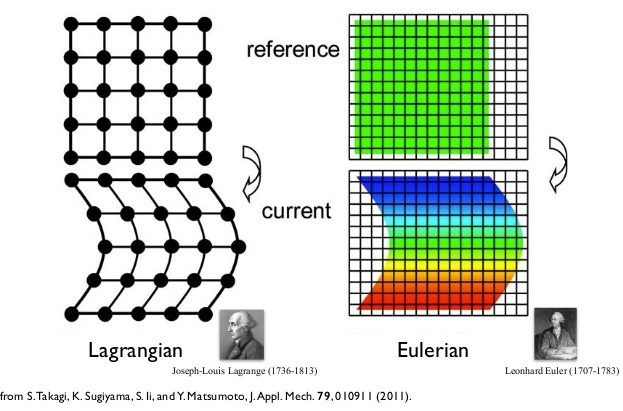
\includegraphics[scale=0.4]{LE2}
	\caption{Blatantly stolen from the internet}
	\label{fig:LE}
\end{figure}
\end{frame}
\section{Overview of Continuum Mechanics}
\begin{frame}{Overview of Continuum Mechanics}
	\begin{figure}
		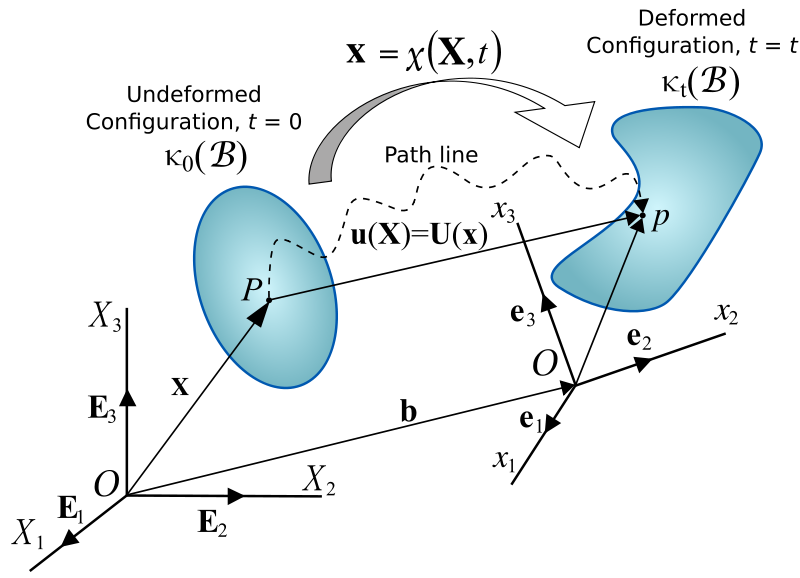
\includegraphics[scale=0.25]{Deform}
		\caption{Deformation (Remember when your teacher told you not to use Wikipedia?)}
	\end{figure}
	
\end{frame}
\begin{frame}{Overview of Continuum Mechanics}
	Let the relationship between the Lagrangian and Eularian coordinates be:
	\begin{subequations}
		\begin{equation}\label{eq:phi}		
			\bm{x}=\bm{\chi}(\bm{X})
		\end{equation}
		\begin{equation}
			d\bm{x}=\frac{\partial \bm{\chi}}{\partial\bm{X}}d\bm{X}
		\end{equation}
		\begin{equation}
			F_{ij}=\frac{\partial \chi_{i}}{\partial X_{j}}
		\end{equation}
	\end{subequations}
\begin{block}{Deformation Gradient}
$\bm{F}$ is known as the \textbf{Deformation Gradient Tensor} and it is probably the most important quantitiy in
continuum mechanics. It relates a material (Lagrangian) infinitesimal vector $\bm{dX}$ to the spatial (Eularian) 
vector $\bm{dx}$. It is very often used in development of constitutive equations and as well as measures of strain. 
For instance the Green-Lagrange Strain Tensor is given by:
\end{block}
\begin{equation}
	\bm{E}=\frac{1}{2}(\bm{F}^{T}\bm{F}-\bm{I})
\end{equation}
\end{frame}

\subsection{Conservation Equations}
\begin{frame}{Conservation Equations}
	The three physical quantities that we are trying to conserve:
	\begin{enumerate}
		\item mass
		\item linear momentum
		\item energy
	\end{enumerate}
\vspace{1cm}
	Each of these conservation equations can be represented withing the Lagrangian or the Eularian Frame 
    work. Keeping in mind that we can always jump between them and they represent the same physical process.
\end{frame}

\subsubsection{Conservation of Mass}
\begin{frame}{Conservation of Mass}
The detailed derivation of this can be found in Belytschko, \textbf{Section 3.5.4}
	\begin{block}{Lagrangian}
		Lagrangian conservation of mass is given by:
		\begin{subequations}
			\begin{equation}
				\rho(\bm{X},t)J(\bm{X},t)=\rho_{0}(\bm{X})
			\end{equation}
			\begin{equation}
				J(\bm{X},t)=det|\bm{F}(\bm{X},t)|
			\end{equation}
		\end{subequations}
	\end{block}
\begin{block}{Eularian}
	Eularian conservation of mass is given by:
	\begin{equation}
		\frac{\partial \rho(\bm{x},t)}{\partial t}+\nabla\cdot[\rho(\bm{x},t)\bm{v}						(\bm{x},t)]=0
	\end{equation}
\end{block}
\end{frame}

\subsubsection{Conservation of Momentum}

\begin{frame}{Conservation of Momentum}
The detailed derivation of this can be found in Belytschko, \textbf{Section 3.5.5}
This is of course nothing but $\bm{F}=m\bm{a}$.
\vspace{0.25cm}
We will need to utilize the concept of body force $\bm{b}(\bm{X/x},t)$
and the Cauchy Tensor $\bm{\sigma}(\bm{x},t)$. Notice that $\bm{\sigma}$ is only defined in the spatial (Eularian) frame.
Stresses require careful treatment with respect to the reference frame. Although this is out of scope of this presentation, 
the 1st Piola Kirchhoff $\bm{P}(\bm{X},t)$ is the stress in the material (Lagrangian) configuration.
\end{frame}

\begin{frame}{Conservation of Momentum}
\begin{block}{Lagrangian}
	\begin{equation}
		\rho(\bm{X},t)\frac{\partial\bm{v}(\bm{X},t)}{\partial t}=\nabla\cdot\bm{\sigma}(\bm{x},t)+\rho(\bm{X},t)\bm{b}(\bm{X},t)
	\end{equation}
    Note that $\bm{\sigma}$ is in the spatial and not the material coordinates
\end{block}

\begin{block}{Eularian}
	\begin{equation}
		\frac{D(\rho\bm{v})}{Dt}=div(\bm{\sigma)}+\rho\bm{b}
	\end{equation}
	For simplicity, the spatial coordinates were omited, but all are functions of $\bm{x}$
\end{block}
\end{frame}

\subsubsection{Conservation of Energy}

\begin{frame}{Conservation of Energy}
These are getting really complicated, so conservation of energy is only shown in the Eularian Frame work.
This is derived in more detail in Belytschko \textbf{Section 3.5.9}
	\begin{equation}
		\rho\frac{Dw^{int}}{Dt}=\bm{D}:\bm{\sigma}-\nabla\cdot\bm{q}+\rho s
	\end{equation}
	Note the use of the velocity gradient $\bm{D}$. The definition of $\bm{D}$ comes from the rate of deformation tensor $\bm{L}$
	\begin{subequations}
		\begin{equation}
			\bm{L}=\dot{\bm{F}}\cdot\bm{F}^{-1}
		\end{equation}
		\begin{equation}
			\dot{\bm{F}}=\frac{\partial \bm{v}}{\partial \bm{X}}
		\end{equation}
		\begin{equation}
			\bm{L}=\frac{1}{2}[\bm{L}+\bm{L}^{T}]+\frac{1}{2}[\bm{L}-\bm{L}^{T}];\
			\bm{L}=\bm{D}+\bm{W}
		\end{equation}
	\end{subequations}
\end{frame}

\section{Developing the Weak Form}
\begin{frame}{Developing the Weak Form}
A few concepts that need to be familiar:
\begin{itemize}
	\item Gauss's Theorem Equation: \ref{eq:div}
	\item Traction Force Vector Equation: \ref{eq:trac}
	\item Virtual Displacement or Velocity $\delta\bm{u}$ or $\delta\bm{v}$
	\end{itemize}
\vspace{1cm}
	\begin{equation}
		\iiint_V\nabla\cdot\bm{F}d\bm{V}=\oint_V \bm{F}\cdot\bm{n}dS
		\label{eq:div}
	\end{equation}
	\begin{equation}
		\bm{t}=\bm{n}\cdot\bm{\sigma}
		\label{eq:trac}
	\end{equation}
\end{frame}

\begin{frame}{Developing the Weak Form}
	We will focus on the momentum equation in developing the weak form. The momentum equation with the boundary conditions is given by \ref{eq:mom} :
	\begin{subequations}
		\begin{equation}
			\frac{\partial \sigma_{ji}}{\partial x_{j}}+\rho b_{i}=\rho \dot{v}_{i}
		\end{equation}
		\begin{equation}
			n_{j}\sigma_{ji}=t_{i}\; on\; \Gamma_{t_{i}}
		\end{equation}
		\begin{equation}
			n_{j}\sigma_{ji}=0\; on\; \Gamma_{int}
		\end{equation}
		\label{eq:mom}
	\end{subequations}
\end{frame}

\begin{frame}{Developing the Weak Form}
	So why bother to convert to the weak form?
	\begin{itemize}
		\item Stresses are functions of velocity or displacement gradients
		\item That means our approximation functions have to be twice differentiable (not ideal)
		\item We seek a form that can be approximated by piecewise linear approximation functions
	\end{itemize}
\end{frame}
\begin{frame}{Developing the Weak Form}
	To obtain the weak form, we multiply by the virtual velocity (because our momentum equation is 
	in terms of velocity) and integrate over the volume to obtain:
	\begin{equation}
		\int_{\Omega}\delta v_{i}\bigg(\frac{\partial \sigma_{ji}}{\partial x_{j}}+\rho b_{i}-\rho\dot{v}_{i}\bigg)d\Omega=0
		\label{eq:virtv}
	\end{equation}
	Applying the product rule:
	\begin{equation}
		\int_{\Omega}\delta v_{i}\bigg(\frac{\partial \sigma_{ji}}{\partial x_{j}}\bigg)d\Omega=
		\int_{\Omega}\bigg[\frac{\partial}{\partial x_{j}}(\delta v_{i} \sigma_{ji})-
		\frac{\partial (\delta v_{i})}{\partial x_{j}}\sigma_{ji}\bigg]d\Omega
		\label{eq:prod}
	\end{equation}
	And Gauss's Theorem along with the boundary condition of \ref{eq:mom}:
	\begin{equation}
		\int_{\Omega}\bigg[\frac{\partial}{\partial x_{j}}(\delta v_{i} \sigma_{ji})\bigg]d\Omega=
		\int_{\Gamma}\delta v_{i} n_{j}\sigma_{ji}d\Gamma=
		\sum_{i=1}^{NSD}\int_{\Gamma}\delta v_{i}\bar{t}d\Gamma
		\label{eq:gauss}
	\end{equation}
	We have used the fact that the boundary term on the internal boundaries is 0
\end{frame}
\subsubsection{Principle of Virtual Power}
\begin{frame}{Principle of Virtual Power}
	When Equation \ref{eq:gauss} is substituted into equation \ref{eq:prod} we obtain:
	\begin{equation}
	\int_{\Omega}\delta v_{i}\frac{\partial \sigma_{ji}}{\partial x_{j}}=
	\int_{\Gamma}\delta v_{i} n_{j}\sigma_{ji}d\Gamma-
	\int_{\Omega}\frac{\partial (\delta v_{i})}{\partial x_{j}}\sigma_{ji}d\Omega
	\label{eq:vp_int}
	\end{equation}
	and Equation \ref{eq:vp_int} is substituted into equation \ref{eq:virtv} we obtain the \textbf{The principal of virtual power}
   \begin{equation}
	   \int_{\Omega}\frac{\partial (\delta v_{i})}{\partial x_{j}}\sigma_{ji}d\Omega-
	   \int_{\Omega}\delta \rho v_{i}d\Omega-
	   \sum_{i=1}^{NSD}\int_{\Gamma}\delta v_{i}\bar{t}d\Gamma+
	   \int_{\Omega}\delta v_{i}\rho\dot{v}_{i}d\Omega=0
   \end{equation}
   This is the equation that most Finite Element codes are solving
\end{frame}

\subsubsection{Shape Functions}
\begin{frame}{Shape Functions}
	So far no numerical approximation has been made. We just wrapped the conservation equations
	in the variational framework by converting to the weak form. 
	We now introduce the linear shape function on the element $N_{I}(\bm{X})$ the map between the 
	material and the spatial coordinate can now be approximated as:
	
	\begin{equation}
		x_{i}(\bm{N},t)=N_{I}(\bm{X})x_{iI}(t)
	\end{equation}
	Note this simple approximation allows us to approximate to calculate quite a bit of information for instance:
	\begin{subequations}
		\begin{equation}
			\bm{F}(\bm{X},t)=\bm{x}_{I}(t)\frac{\partial \bm{N}_{I}}{\partial \bm{X}}
		\end{equation}
		\begin{equation}
			\bm{L}=\bm{v}_{I}\frac{\partial \bm{N}_{I} }{\partial \bm{x}}\bm{F}^{-1}=
			\dot{\bm{F}}\bm{F}^{-1}
		\end{equation}
	\end{subequations}
\end{frame}
\section{Outro}
\begin{frame}{Outro}
	This is all the Finite Element stuff we will go over today, but feel free to stop by my office and ask questions. I encourage you to read through Belytschko's book. You can leaf through my copy in the mean time
\end{frame}


\end{document}
